% ***********************************************************
% ******************* PHYSICS HEADER ************************
% ***********************************************************
% Version 2
\documentclass[11pt]{article}
\usepackage{amsmath} % AMS Math Package
\usepackage{amsthm} % Theorem Formatting
\usepackage{amssymb}	% Math symbols such as \mathbb
\usepackage{graphicx} % Allows for eps images
\usepackage{multicol} % Allows for multiple columns
\usepackage[dvips,letterpaper,margin=0.75in,bottom=0.5in]{geometry}
\usepackage{authblk} % Allows for authors from multiiple institutes
\renewcommand\Authands{ and } % for authblk
\usepackage{indentfirst} % to have indent for the 1st paragraph of each section

 % Sets margins and page size
\pagestyle{empty} % Removes page numbers

\makeatletter % Need for anything that contains an @ command

\newcommand{\affil}[1]{\def\@affilname{#1}}
\def\@affil{\@affilname}

\renewcommand{\maketitle} % Redefine maketitle to conserve space
{ \begingroup \vskip 10pt \begin{center} \large {\textbf{\@title}}
\vskip 10pt \large \@author \vskip 10pt \large \@affil \end{center}
\vskip 10pt \endgroup \setcounter{footnote}{0} }

\makeatother % End of region containing @ commands
\renewcommand{\labelenumi}{(\alph{enumi})} % Use letters for enumerate
% \DeclareMathOperator{\Sample}{Sample}
\let\vaccent=\v % rename builtin command \v{} to \vaccent{}
\renewcommand{\v}[1]{\ensuremath{\mathbf{#1}}} % for vectors
\newcommand{\gv}[1]{\ensuremath{\mbox{\boldmath$ #1 $}}}
% for vectors of Greek letters
\newcommand{\uv}[1]{\ensuremath{\mathbf{\hat{#1}}}} % for unit vector
\newcommand{\abs}[1]{\left| #1 \right|} % for absolute value
\newcommand{\avg}[1]{\left< #1 \right>} % for average
\let\underdot=\d % rename builtin command \d{} to \underdot{}
\renewcommand{\d}[2]{\frac{d #1}{d #2}} % for derivatives
\newcommand{\dd}[2]{\frac{d^2 #1}{d #2^2}} % for double derivatives
\newcommand{\pd}[2]{\frac{\partial #1}{\partial #2}}
% for partial derivatives
\newcommand{\pdd}[2]{\frac{\partial^2 #1}{\partial #2^2}}
% for double partial derivatives
\newcommand{\pdc}[3]{\left( \frac{\partial #1}{\partial #2}
 \right)_{#3}} % for thermodynamic partial derivatives
\newcommand{\ket}[1]{\left| #1 \right>} % for Dirac bras
\newcommand{\bra}[1]{\left< #1 \right|} % for Dirac kets
\newcommand{\braket}[2]{\left< #1 \vphantom{#2} \right|
 \left. #2 \vphantom{#1} \right>} % for Dirac brackets
\newcommand{\matrixel}[3]{\left< #1 \vphantom{#2#3} \right|
 #2 \left| #3 \vphantom{#1#2} \right>} % for Dirac matrix elements
\newcommand{\grad}[1]{\gv{\nabla} #1} % for gradient
\let\divsymb=\div % rename builtin command \div to \divsymb
\renewcommand{\div}[1]{\gv{\nabla} \cdot #1} % for divergence
\newcommand{\curl}[1]{\gv{\nabla} \times #1} % for curl
\let\baraccent=\= % rename builtin command \= to \baraccent
\renewcommand{\=}[1]{\stackrel{#1}{=}} % for putting numbers above =
\newtheorem{prop}{Proposition}
\newtheorem{thm}{Theorem}[section]
\newtheorem{lem}[thm]{Lemma}
\theoremstyle{definition}
\newtheorem{dfn}{Definition}
\theoremstyle{remark}
\newtheorem*{rmk}{Remark}

\usepackage[english]{babel}
\graphicspath{{images/}}
\usepackage{siunitx}
\usepackage{lineno}

\def\lycoris{\textsc{Lycoris }}%
\def\GeV{\ifmode {\mathrm{\ Ge\kern -0.1em V }}\else
								 {\textrm{Ge\kern -0.1em V }}\fi}%

% ***********************************************************
% ********************** END HEADER *************************
% ***********************************************************


\begin{document}

\title{\textsc{Lycoris}: A large area beam telescope based on hybrid-less strip silicon sensors}
\author[*]{Mengqing Wu}
\author[*]{Uwe Kraemer}
\author[*]{Marcel Stanitziki}
\author[**]{Martin Breidenbach}
\author[**]{Dietrich R. Freytag}
\author[**]{Benjamin A. Reese}
\affil[*]{Deutsches Elektronen-Synchrotron DESY, Notkestr. 85, 22607 Hamburg, Germany}
\affil[**]{Stanford Linear Accelerator Center SLAC, 2575 Sand hill Rd, Menlo Park, CA 94025 USA}

\maketitle

\begin{abstract}
%\linenumbers

A new Large area x-Y COverage Readout Integrated Strip telescope (\lycoris),
is being built as an improvement of the DESY test beam infrastructure within the Advanced European Infrastructures for Detectors at Accelerators project (AIDA-2020).
The \lycoris telescope consists of 6 layers of 10$\times$\SI{10}{\square\centi\metre} strip sensors with a pitch of \SI{25}{\micro\metre};
it is designed to provide a spatial resolution better than \SI{10}{\micro\metre} along the bending direction,
will be mounted inside a superconducting solenoid magnet of \SI{1}{\tesla},

to provide a spatial resolution better than
and a resolution better than \SI{1}{\milli\meter} along the magnetic field.
The full readout system was tested with a hexagonal pixel sensor in the lab with a Sr90 source,
and later tested in the DESY test beam with minimum electron energy of \SI{4}{\GeV}.

The telescope is expected to be delivered at the beginning of 2019 with a complete package,
including its own hardware with a common readout system, a new AIDA2020-type TLU and a reconstruction software for user.
Therefore, a first user case, LP-TPC, to complete R&D is in schedule in fall 2018. In this talk, the current project status with latest results will be shown.

\end{abstract}

\section*{A large active area beam telescope}
%\linenumbers

The AHCAL barrel for the ILC is a cylindrical structure with an inner radius of \SI{1.8}{\metre} and outer radius of \SI{2.8}{\metre}.
Inside the AHCAL, an electromagnetic calorimeter (ECAL) will be placed while the AHCAL will be surrounded by the coil magnet. The circular structure is divided into 16 segments containing 48 layers each. An AHCAL layer consists of an HCAL Base Unit (HBU) of 36$\times$\SI{36}{\square\centi\metre} with 144 scintillating tiles of 3$\times$3$\times$\SI{0.3}{\cubic\centi\metre} connected to SiPMs readout by 4 ASICs. The active layers will be placed between \SI{2}{\centi\metre} thick absorber plates of steel. A complete layer contains 2592 channels which for the complete barrel adds up to 3.9 million of channels. The complete AHCAL including the endcaps will add up to 8 million channels.\\

The ASICs include several features: digitization integrated into the front-end, on-detector zero suppression, channel-wise pre-amplifiers to compensate the spread in SiPM gains and channel-wise voltage bias (DACs) are foreseen to compensate the spread in SiPM operating voltages allowing to operate the detector with a single threshold for all channels on an ASIC. In addition here, the front-end has the capability of measuring timing via a voltage ramp (TDC) at single channel level allowing to study the time development of showers and the identification of late particles in harden shower, mostly thermal neutrons.\\

\begin{figure}[!ht]%
\centering
\vspace{-10px}
\hspace{-100px}
\parbox{1.2in}{
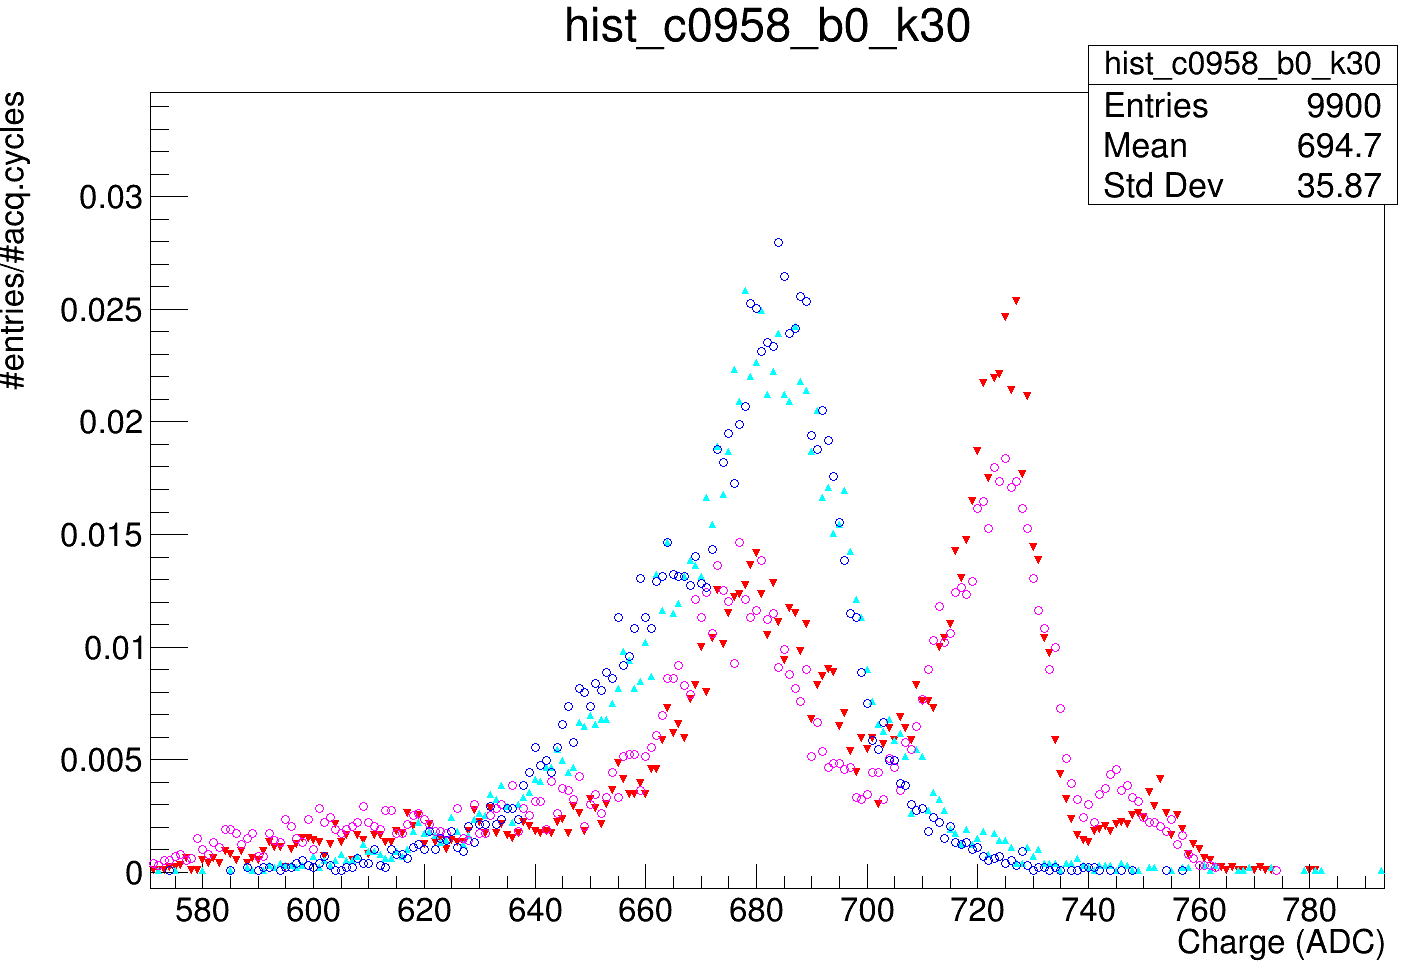
\includegraphics[width=2.5\linewidth, trim={1cm 9cm 3cm 5cm}, clip]{pics/hardware1.png}
}%
\hspace{150px}
\begin{minipage}{1.2in}%
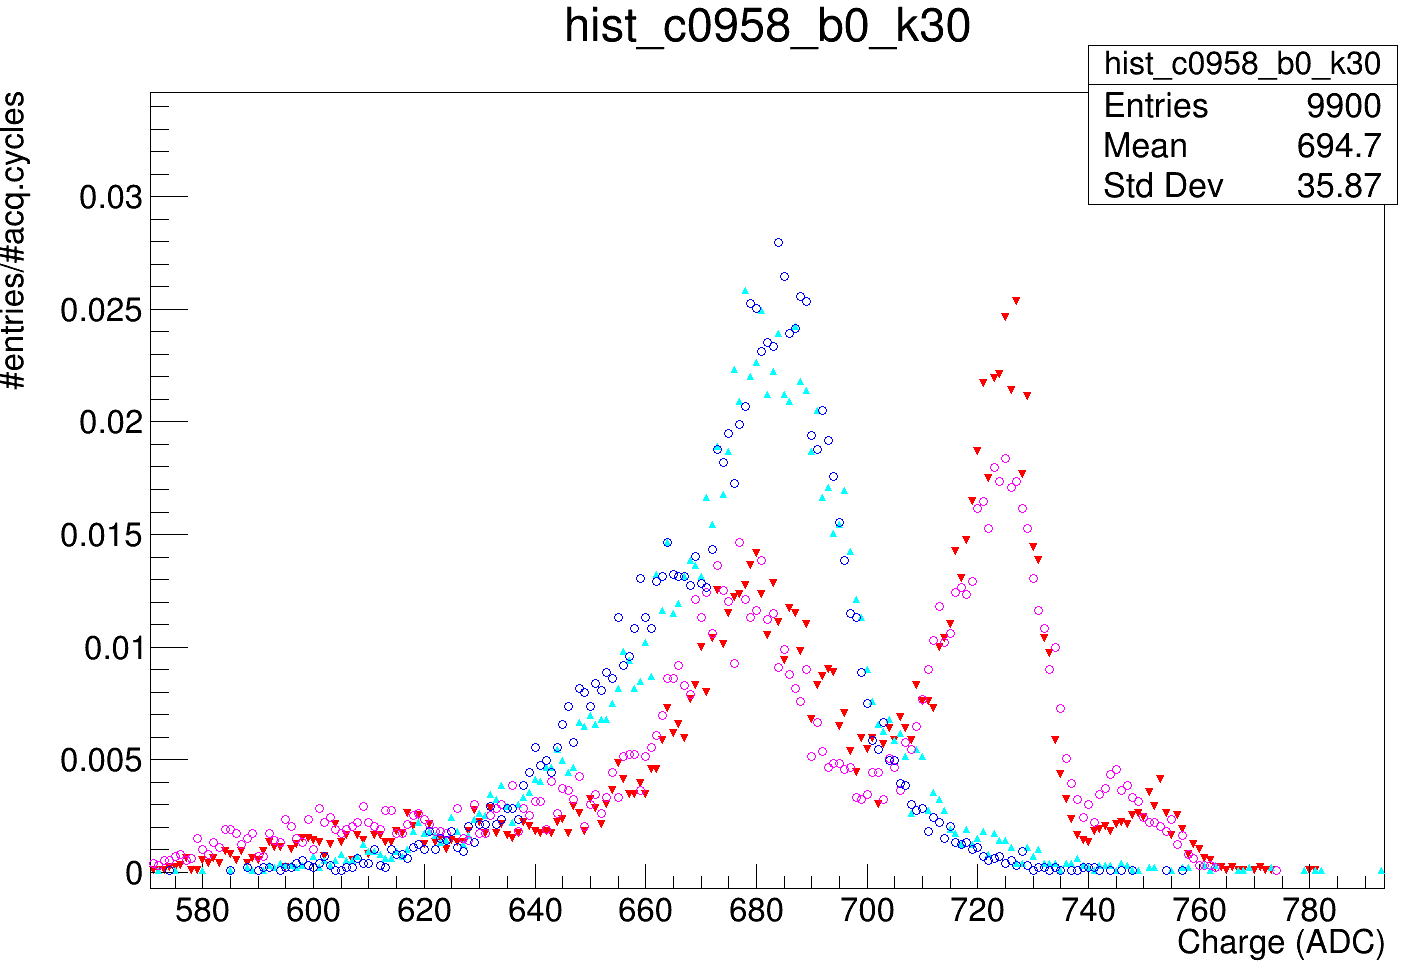
\includegraphics[width=2.2\linewidth]{pics/hardware1.png}
\end{minipage}%
\caption{On the left, testbeam setup used at the CERN SPS in Summer 2015. On the right, picture of the AHCAL testbeam prototype used at the CERN SPS in Summer 2015. The front face of the calorimeter is on the right of the picture.}%
\label{fig:1figs}%
\end{figure}

A multi-layer prototype (see fig.\ref{fig:1figs}) was commissioned in summer 2014; it is containing up to 15 active layers. The first 2 layers consisted of ECAL Base Units (EBU) of 18$\times$\SI{18}{\square\centi\metre} with 144 scintillating strips of 4.5$\times$0.5$\times$\SI{0.2}{\cubic\centi\metre} equipped with MPPCs of 10k and 1.6k pixels respectively, and the same electronics as the previously described HBUs. The next 8 layers consisted of HBUs with 144 channels, equipped with several different types of scintillator tile designs and SiPMs. The main goal of these first layers is the localisation of the first hard interaction in a hadronic shower. The last 4 layers each consisted of 4 HBUs in a 2 by 2 configuration (72$\times$\SI{72}{\square\centi\metre}) having 576 channels. The first two of them were equipped with Ketek SiPMs (2.3k pixels), and the other two with SenSL SiPMs (1.3k pixels). The layers were arranged in a way to study timing correlations with the two first layers close to each other while the two last layers were further separated from each other.

\begin{figure}[!ht]%
\centering
\vspace{-80px}
\hspace{-80px}
\parbox{1.2in}{
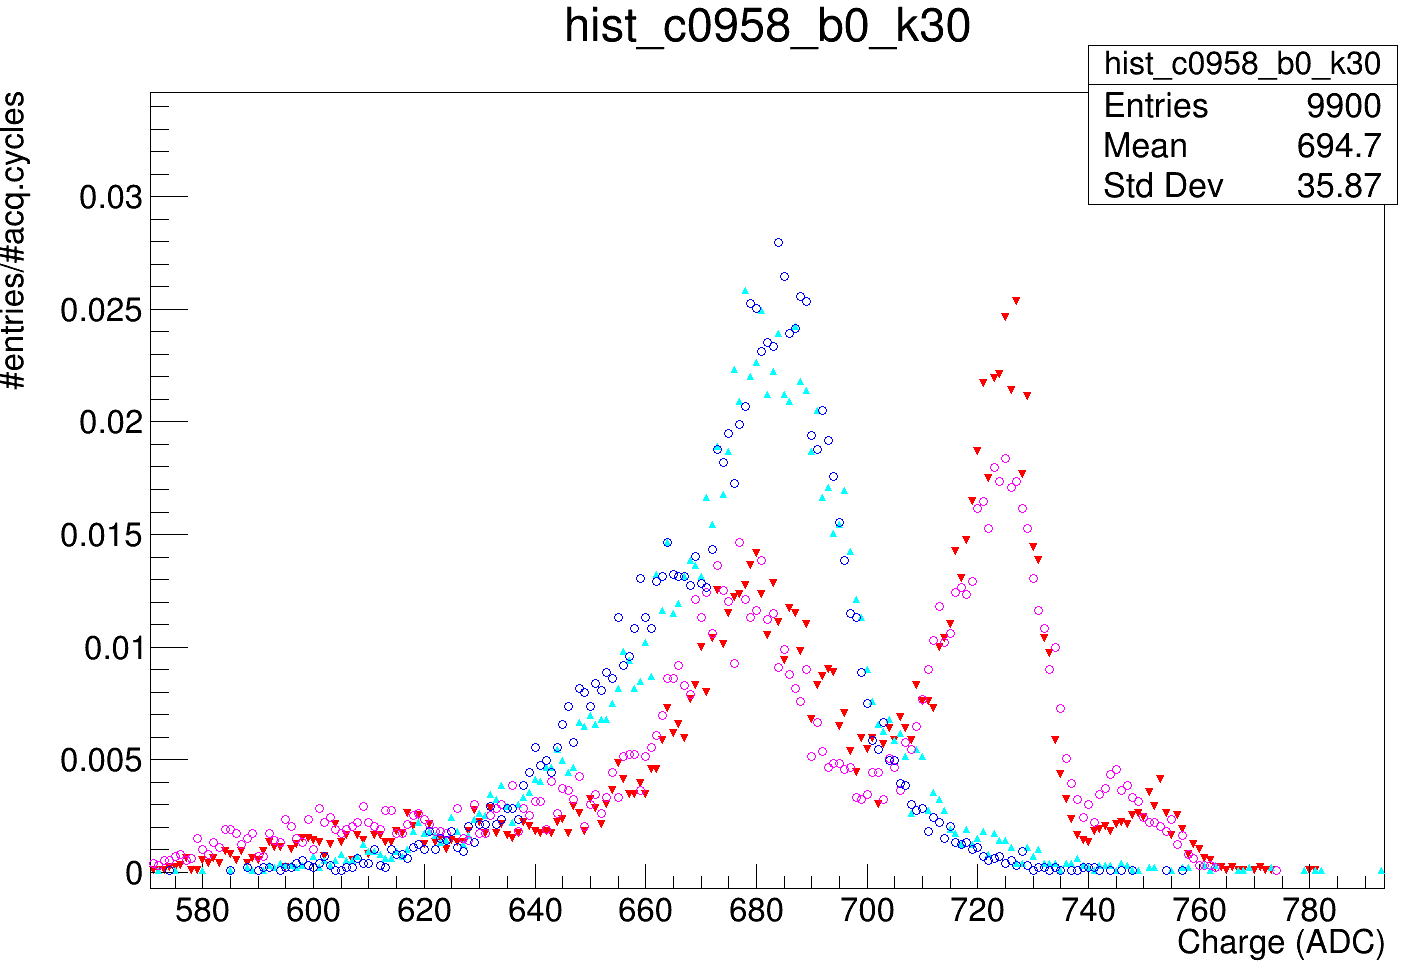
\includegraphics[width=2.5\linewidth]{pics/hist1.jpg}
}%
\hspace{150px}
\begin{minipage}{1.2in}%
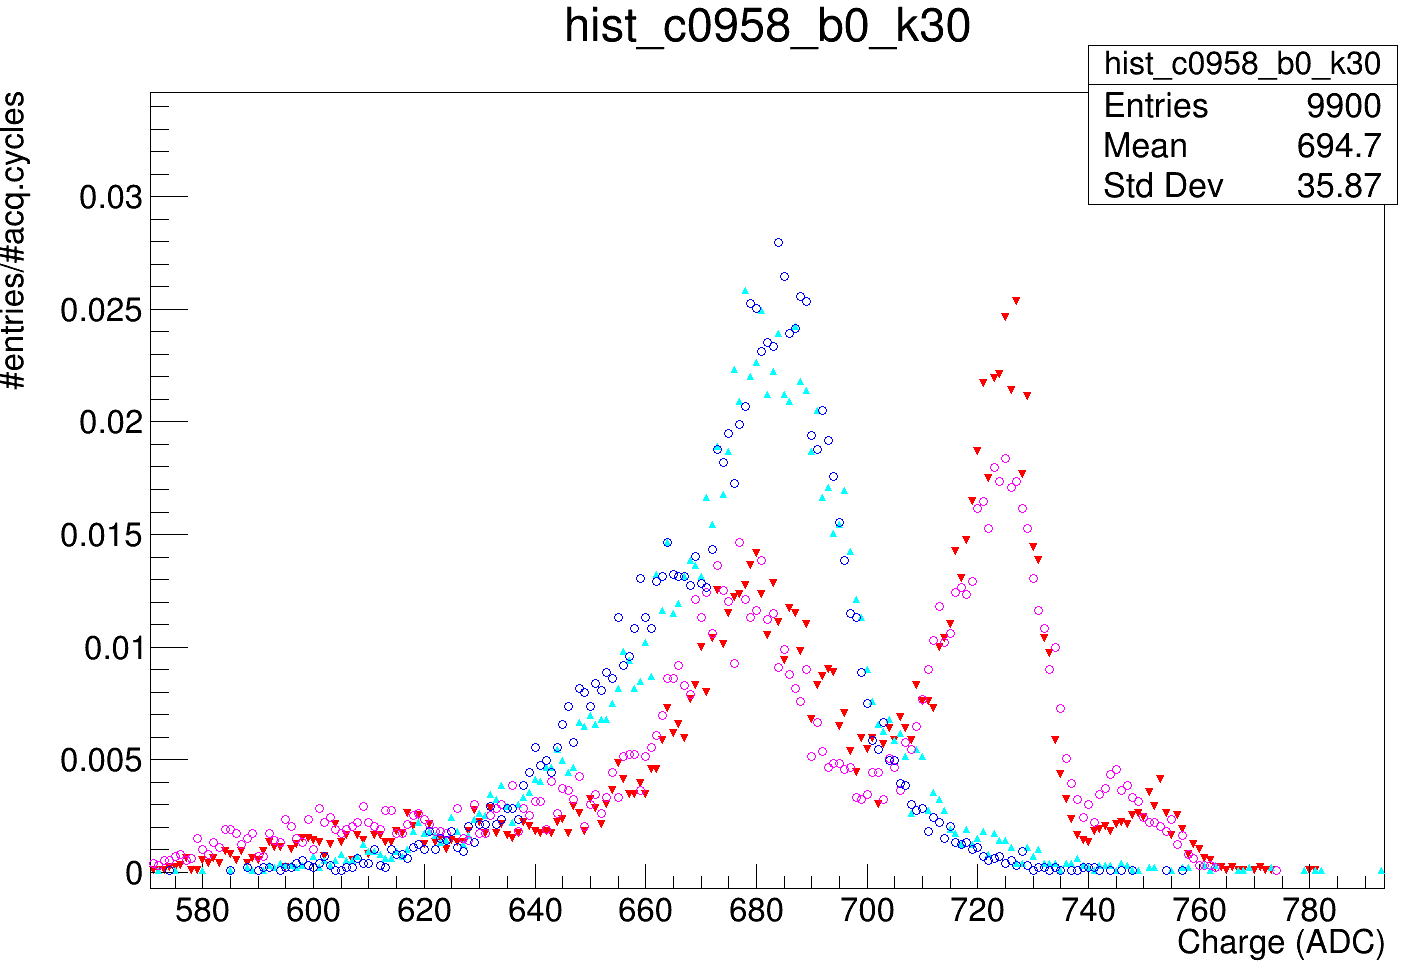
\includegraphics[width=1.4\linewidth]{pics/hist1.jpg}
\end{minipage}%
\vspace{-80px}
\caption{Minimum ionising particle energy spectra of a typical channel of the AHCAL prototype after energy calibration. On the right, simplified schematics of the TDC voltage ramp in the SPIROC2b ASIC for both testbeam and ILC mode.}%
\label{fig:2figs}%
\end{figure}

Timing development of hadronic shower has already been studied in CALICE using the TungstenTiming TestBeam set-up (T3B)$^{\cite{T3B}}$. The study showed that hadronic showers have a time development that is very sensitive to the absorber material. It is characterised by 3 major contributions: instantaneous energy deposition mostly due to the electromagnetic component in the shower core, and a medium/late contribution mostly due to thermal neutrons traveling through the detector and extending into the halo (from few ns to hundreds of ns). Thus a better separation of nearby showers using timing information to identify late neutrons could improve jet energy resolution in the PFA. In addition to the test of different sensor configurations, the goal of the test beam experiment is to investigate such possibilities with real data.

After the energy calibration of the detector to the MIP scale, a timing calibration of the detector has to be performed (see fig.\ref{fig:2figs}). To convert the TDC value to a time value in ns, a conversion slope has to be calibrated as well as a pedestal. The TDC slope depends on the frequency used to operate the detector, in testbeam, the frequency used is 250 kHz (4 $\mu$s). The expected timing resolution for the AHCAL in testbeam is around 4-5 ns precision. For ILC, the expected resolution is under 1 ns.
In this contribution, we will describe the timing calibration procedure, and we will present the first results on timing resolution with muon and electron beams obtained in testbeam data and compare them to simulation.

\footnotesize
\begin{thebibliography}{1}

\bibitem{T3B} The CALICE Collaboration, C. Adloff et al., {\em The time structure of hadronic showers in highly granular calorimeters with tungsten and
steel absorbers}, \textbf{2014 JINST 9 P07022}.

\end{thebibliography}

\end{document}
